\usepackage{amsmath}\documentclass{book}

\usepackage{fontspec}
\setmainfont{Ubuntu}

\usepackage[left=1in, right=1in, top=1in, bottom=1in]{geometry}

\usepackage{fancyhdr}
\pagestyle{fancy}
\lhead{\href{https://github.com/QubitPi/general-relativity}{Supplementary Study Notes }}
\chead{General Relativity}
\rhead{
    \href{https://github.com/QubitPi}{QubitPi}
    
\includegraphics[scale=0.05]{logo-8th-version.png}
}
\lfoot{}
\cfoot{}
\rfoot{\thepage}
\renewcommand{\headrulewidth}{0.4pt}
\renewcommand{\footrulewidth}{0.4pt}

\usepackage{hyperref}
\hypersetup{
    colorlinks=true,
    linkcolor=blue,
    anchorcolor=blue,
    urlcolor=blue
}

\usepackage{graphicx}
\usepackage{float}
\graphicspath{ {./img/} }
\usepackage{tikz}
\usepackage[most]{tcolorbox}


\newtcbtheorem[number within=section]{mytheorem}{Theorem}
{colback=green!5,colframe=green!35!black}{th}

\newtcbox{\roundinlinebox}[1][red]{on line,
arc=7pt,colback=#1!10!white,colframe=#1!50!white,
before upper={\rule[-3pt]{0pt}{10pt}},boxrule=1pt,
boxsep=0pt,left=6pt,right=6pt,top=2pt,bottom=2pt}

% https://tex.stackexchange.com/a/307436/277953
\newtcolorbox{marker}[1][]{enhanced,
before skip=2mm,after skip=3mm,
boxrule=0.4pt,left=5mm,right=2mm,top=1mm,bottom=1mm,
colback=yellow!50,
colframe=yellow!20!black,
sharp corners,rounded corners=southeast,arc is angular,arc=3mm,
underlay={%
    \path[fill=tcbcolback!80!black] ([yshift=3mm]interior.south east)--++(-0.4,-0.1)--++(0.1,-0.2);
    \path[draw=tcbcolframe,shorten <=-0.05mm,shorten >=-0.05mm] ([yshift=3mm]interior.south east)--++(-0.4,-0.1)--++(0.1,-0.2);
    \path[fill=yellow!50!black,draw=none] (interior.south west) rectangle node[white]{\Huge\bfseries !} ([xshift=4mm]interior.north west);
},
drop fuzzy shadow,#1}

\usepackage{amsfonts}
\usepackage{parskip}

\setlength{\parindent}{0pt}

\usepackage{xcolor}
\usepackage{framed}
\usepackage{titletoc}
\usepackage{etoolbox}

% definition of some personal colors
\definecolor{myred}{RGB}{127,0,0}
\definecolor{myyellow}{RGB}{169,121,69}

% command for the circle for the number of part entries
\newcommand\Circle[1]{\tikz[overlay,remember picture]
    \node[draw,circle, text width=18pt,line width=1pt] {#1};}

% patching of \tableofcontents to use sans serif font for the tile
\patchcmd{\tableofcontents}{\contentsname}{\contentsname}{}{}
% patching of \@part to typeset the part number inside a framed box in its own line
% and to add color
\makeatletter
\patchcmd{\@part}
{\addcontentsline{toc}{part}{\thepart\hspace{1em}#1}}
{\addtocontents{toc}{\protect\addvspace{20pt}}
    \addcontentsline{toc}{part}{\huge{\protect\color{myyellow}%
        \setlength\fboxrule{2pt}\protect\Circle{%
            \hfil\thepart\hfil%
        }%
    }\\[2ex]\color{myred}#1}}{}{}

%\patchcmd{\@part}
%  {\addcontentsline{toc}{part}{\thepart\hspace{1em}#1}}
%  {\addtocontents{toc}{\protect\addvspace{20pt}}
%    \addcontentsline{toc}{part}{\huge{\protect\color{myyellow}%
%      \setlength\fboxrule{2pt}\protect\fbox{\protect\parbox[c][1em][c]{1.5em}{%
%        \hfil\thepart\hfil%
%      }}%
%    }\\[2ex]\color{myred}#1}}{}{}
\makeatother

% this is the environment used to typeset the chapter entries in the ToC
% it is a modification of the leftbar environment of the framed package
\renewenvironment{leftbar}
{\def\FrameCommand{\hspace{6em}%
{\color{myyellow}\vrule width 2pt depth 6pt}\hspace{1em}}%
    \MakeFramed{\parshape 1 0cm \dimexpr\textwidth-6em\relax\FrameRestore}\vskip2pt%
}
{\endMakeFramed}

% using titletoc we redefine the ToC entries for parts, chapters, sections, and subsections
\titlecontents{part}
[0em]{\centering}
{\contentslabel}
{}{}
\titlecontents{chapter}
[0em]{\vspace*{2\baselineskip}}
{\parbox{4.5em}{%
    \hfill\Huge\bfseries\color{myred}\thecontentspage}%
    \vspace*{-2.3\baselineskip}\leftbar\textsc{\small\chaptername~\thecontentslabel}\\}
{}{\endleftbar}
\titlecontents{section}
[8.4em]
{\contentslabel{3em}}{}{}
{\hspace{0.5em}\nobreak\itshape\color{myred}\contentspage}
\titlecontents{subsection}
[8.4em]
{\contentslabel{3em}}{}{}
{\hspace{0.5em}\nobreak\itshape\color{myred}\contentspage}


\begin{document}

    \listoftodos

    \pgfornament[width=5cm]{80}

    \begin{tcolorbox}[breakable,enhanced jigsaw,title={Contents},fonttitle=\bfseries\Large,
    colback=yellow!10!white,colframe=red!50!black,before=\par\bigskip\noindent,
    interior style={fill overzoom image=goldshade.png,fill image opacity=0.25},
    colbacktitle=red!50!yellow!75!black,
    enlargepage flexible=\baselineskip,pad at break*=3mm,
    watermark color=yellow!75!red!25!white,
    watermark text={\bfseries\Large Contents},
    attach boxed title to top center={yshift=-0.25mm-\tcboxedtitleheight/2,yshifttext=2mm-\tcboxedtitleheight/2},
    boxed title style={enhanced,boxrule=0.5mm,
    frame code={ \path[tcb fill frame] ([xshift=-4mm]frame.west) -- (frame.north west)
        -- (frame.north east) -- ([xshift=4mm]frame.east)
        -- (frame.south east) -- (frame.south west) -- cycle; },
    interior code={ \path[tcb fill interior] ([xshift=-2mm]interior.west)
        -- (interior.north west) -- (interior.north east)
        -- ([xshift=2mm]interior.east) -- (interior.south east) -- (interior.south west)
        -- cycle;}  },
    drop fuzzy shadow]
        \makeatletter
        \@starttoc{toc}
        \makeatother
    \end{tcolorbox}

    \part{\href{https://trello.com/c/jzmmeXHp}{A First Course on General Relativity}}
    \chapter{Special Relativity}
    \section{Einstein's Original Paper on ``Special Relativity"}

\begin{marker}
    This section is not from the book, but simply my extra interests on the history of SR
\end{marker}

\begin{tcolorbox}[
    colback=green!5!white,
    colframe=green!75!black,
    colbacktitle=red!85!black
]
    \phantomsection\hypertarget{sr-original-paper}
    The original paper is in \href{https://trello.com/c/ll9Yzd8h}{The Collected Papers of Albert Einstein, Vol.2}, page 140, \textit{On the Electrodynamics of Moving Bodies}
\end{tcolorbox}

Reading the original paper requires the prerequisites of

\begin{itemize}
    \item \href{https://en.wikipedia.org/wiki/Michelson\%E2\%80\%93Morley\_experiment}{Michelson-Morley Experiment}

          \begin{itemize}
              \item \href{https://youtu.be/3G_Q6AggQF8?si=ihpGM23NGq2PfsE2}{An excellent experiment intro}
              \item What I care most about this experiment is the \textbf{way we handle "unsolvable" problems}. Michelson-Morley
              experiment had led to extensive followups trying to explain what was seen in the experiment. All the
              \textit{mediocre} conclusion simply said: "Dude, we don't know." Albert Einstein innovated a new era of Physics out of this conflict. \textbf{When a problem seems to lead to a dead end, it's time to innovate; it's time to take on the risk and bring the human into a new world of new opportunities!}
          \end{itemize}

    \item \href{https://trello.com/c/SlPIXwCY}{Maxwell's Electrodynamics}

          \begin{tcolorbox}[
              colbacktitle=red!10!white,
              colback=blue!10!white,coltitle=red!70!black,
              title=Does the Electromagnetic Field \textit{physically} exist?
          ]
              ``There exists a model of the universe which includes a field known as the Electromagnetic Field. This
              model does a remarkably good job of predicting the observations we make in the world. It does so good at
              making such predictions that it is often phrased as 'existing in the
              world"\footnote{\href{https://philosophy.stackexchange.com/a/28010}{https://philosophy.stackexchange.com/a/28010}}
          \end{tcolorbox}
\end{itemize}

\subsection{Reading Notes...}

...of \hyperlink{sr-original-paper}{the Paper}

\subsubsection{Definition of Simultaneity}

\begin{tcolorbox}[enhanced,colframe=green!75!black,colback=green!5!white, title=Definition of ``Simultaneity"]
    If an event occurs at $(t, x, y, z)$, then all observers would see this event at $(t, x', y', z')$, where
    $x \ne x'$, $y \ne y'$, and $y \ne y'$
\end{tcolorbox}

This definition is ideal but proves to be inefficient if we are going to look at a series of events happening one after
another, according to Einstein, because light takes time to travel. But two clocks can \textit{synchronize} in the
following way:

Suppose an event occurs at $A$ and a ray of light leaves from $A$ toward $B$ at $t_A$; the light is reflected from $B$
towards $A$ at $t_B$, and arrives back at $A$ at $t'_A$. The two clocks at $A$ and $B$ satisfies

\[
    t_B - t_A = t'_A - t_B
\]

which means

\begin{equation}\label{eq:tb-by-ta}
    t_B = \frac{t'_A + t_A}{2}
\end{equation}

Imagine a person holding a watch and manages to precisely record $t_A$ and $t'_A$, they will be able to state with
perfect confidence that any other person (or observer) at arbitrary location $B$ sees their event at time $t_B$, which
can be calculated by Eq.\ref{eq:tb-by-ta}, where both $t_A$ and $t'_A$ can be read at that person's hand watch

\begin{tcolorbox}[enhanced,colframe=green!75!black,colback=green!5!white, title=Definition of ``Synchronism"]
    Suppose a ray of light leaves from $A$ toward $B$ at ``A-time" at $t_A$, is reflected from $B$ toward $A$ at
    ``B-time" $t_B$, and arrives back at $A$ at ``A-time" $t'_A$. The two clocks are \textit{synchronous} by defintion
    if

    \begin{equation}
        t_B - t_A = t'_A - t_B
    \end{equation}
\end{tcolorbox}

If follows naturally that

\begin{enumerate}
    \item If the clock in $B$ is synchronous with the clock in $A$, then the clock in $A$ is synchronous with the clock
          in $B$
    \item If the clock in $A$ is synchronous with the clock in $B$ as well as with the clock in $C$, then the clocks in
          $B$ and $C$ are also synchronous relative to each other
\end{enumerate}

The \textbf{speed of light as a universal constant in empty space is thus}:

\begin{tcolorbox}[enhanced,colframe=green!75!black,colback=green!5!white]
    \begin{equation}
        c = \frac{2\overline{AB}}{t'_A - t_A}
    \end{equation}
\end{tcolorbox}

and there is a BIG assumption: all clocks are at \textit{rest} in a system at \textit{rest}

With that, we have a pretty good mechanism to talk about series of events in a system happening at different time,
because we know how to synchronize them 
\includegraphics[height=0.05\textwidth]{可莉-35.png}

\section{Fundamental principles of special relativity theory (SR)}

\subsection{On ``Principle of relativity (Galileo)"}

\subsubsection{Galilean invariance}

\href{https://en.wikipedia.org/wiki/Newton\%27s_laws_of_motion}{Newton's laws of motion} hold in all frames related
to one another by a \href{https://en.wikipedia.org/wiki/Galilean\_transformation}{Galilean transformation}. In
other words, all frames related to one another by such a transformation are inertial (meaning, Newton's equation of
motion is valid in these frames).\footnote{\href{https://en.wikipedia.org/wiki/Galilean_invariance}{Galilean invariance}}
The proof has been given by the book on page 2.

\section{Construction of the coordinates used by another observer}

\subsection{Why would the tangent of the angle is the speed in Fig. 1.2?}

Suppose $\mathcal{O}$ and $\mathcal{\bar{O}}$ both start out at the same position where $\mathcal{\bar{O}}$
moves along the $x$ at some speed. After $t_1$, observer $\mathcal{O}$ sees $\mathcal{\bar{O}}$ at position $x_1$:

\[ \mathcal{\bar{O}}_1 = (x_1, t_1) \]

Observer  $\mathcal{\bar{O}}$, however, still sees themself at $x = 0$:

\[ \mathcal{\bar{O}}_1 = (0, t_1) \]

By definition where ``$\bar{t}$ is the locus of events at constant $\bar{x} = 0$", $\bar{t}$ is the straight line
that passes the origin and the $(x_1, t_1)$:

\begin{tikzpicture}[scale=1.5]
    \draw[->] (-3,0) node[left] (w) {}--(5,0) node[right] (x) {x};
    \draw[->] (0,-3) node[below] (s) {}--(0,5) node[above] (t) {t};
    \draw[line width=.5pt] (.25,-.25) rectangle (-.25,.25) node (o) {};
    \draw[line width=.5] (o)--(135:1) node[above] () {$\mathcal{\bar{O}}_0$, $\mathcal{O}_0$};

    \draw[black,line width=2pt,->] (0,0)--(4,4) node[above] (t-bar) {{$\bar{t}$}};

    \draw[dashed,line width=.5] (3,0) node[below] (x1) {$x_1$} --(3,3);
    \draw[dashed,line width=.5] (0,3) node[left] (t1) {$t_1$} --(3,3);
    \draw[line width=.5pt] (2.75,3.25) rectangle (3.25,2.75) node (f) {};
    \draw (f) node[right] {$(x_1, t_1)$};

    \draw [blue,thick,domain=225:270] plot ({3 + cos(\x)}, {3 + sin(\x)}) node (speed) {};
    \draw (2.5, 1.8) node[right] (speed) {Tangent of this angle is $\bar{v}$};
\end{tikzpicture}

\section{Invariance of the interval}

\begin{tcolorbox}[
    colback=green!5!white,
    colframe=green!75!black,
    colbacktitle=red!30!white,
    title={Why $(\Delta x)^2 + (\Delta y)^2 + (\Delta z)^2 - (\Delta t)^2 = 0$ for two events in the same light beam?}
    \phantomsection\hypertarget{zero-interval}
]

    Let's say, in a simplified 1D case, event $\mathcal{E} = (x_0, t_0)$ and $\mathcal{P} = (x_1, t_1)$.

    \[ (\Delta x)^2 - (\Delta t)^2 = (x_1 - x_0)^2 - (t_1 - t_0)^2 \]

    Since the speed of light is 1,

    \[ (x_1 - x_0)^2 - (t_1 - t_0)^2 = (x_1 - x_0)^2 - (t_1 \times 1 - t_0 \times 1)^2 = (x_1 - x_0)^2 - (x_1 - x_0)^2 = 0 \]
\end{tcolorbox}

\begin{tcolorbox}[
    colback=green!5!white,
    colframe=green!75!black,
    colbacktitle=red!85!black,
    enhanced,
    attach boxed title to top center={yshift=-2mm},
    title={
        \parbox{10cm}{
            Why does the equation contains only $\boldsymbol{M}_{\alpha\beta} + \boldsymbol{M}_{\beta\alpha}$ terms when $\alpha \ne \beta$, which guarantees $\boldsymbol{M}_{\alpha\beta} = \boldsymbol{M}_{\beta\alpha}$?
        }
    }]

    \[
        \Delta\bar{s}^2 = \sum_{\alpha = 0}^3\sum_{\beta = 0}^3 \boldsymbol{M}_{\alpha\beta}\left(\Delta x^{\alpha}\right)\left(\Delta x^{\beta}\right)
    \]
\end{tcolorbox}

Before spending too much time on expanding the equation, we can pick up a pair of indices of
$(\alpha, \beta) = (\alpha^*, \beta^*)$ where $\alpha^* \ne \beta^*$. Then we would definitely have the following 2
terms in the expansion:

\[ \boldsymbol{M}_{\alpha^*\beta^*}\left(\Delta x^{\alpha^*}\right)\left(\Delta x^{\beta^*}\right) \]
\[ \boldsymbol{M}_{\beta^*\alpha^*}\left(\Delta x^{\beta^*}\right)\left(\Delta x^{\alpha^*}\right) \]

Since

\[ \left(\Delta x^{\alpha^*}\right)\left(\Delta x^{\beta^*}\right) = \left(\Delta x^{\beta^*}\right)\left(\Delta x^{\alpha^*}\right) \]

We can then group these 2 terms and factor out the product, leaving

\[
    \left(\Delta x^{\alpha^*}\right)\left(\Delta x^{\beta^*}\right)\left( \boldsymbol{M}_{\alpha^*\beta^*} + \boldsymbol{M}_{\beta^*\alpha^*} \right)
\]

The terms of expanded $\Delta\bar{s}^2$ can be expressed in a matrix of

\[
    \renewcommand{\arraystretch}{4}
    \begin{bmatrix}
        \boldsymbol{M}_{00}\Delta x^0\Delta x^0 & \boldsymbol{M}_{01}\Delta x^0\Delta x^1 & \boldsymbol{M}_{02}\Delta x^0\Delta x^2  & \boldsymbol{M}_{03}\Delta x^0\Delta x^3 \\
        \boldsymbol{M}_{10}\Delta x^1\Delta x^0 & \boldsymbol{M}_{11}\Delta x^1\Delta x^1 & \boldsymbol{M}_{12}\Delta x^1\Delta x^2  & \boldsymbol{M}_{13}\Delta x^1\Delta x^3 \\
        \boldsymbol{M}_{20}\Delta x^2\Delta x^0 & \boldsymbol{M}_{21}\Delta x^2\Delta x^1 & \boldsymbol{M}_{22}\Delta x^2\Delta x^2  & \boldsymbol{M}_{23}\Delta x^2\Delta x^3 \\
        \boldsymbol{M}_{30}\Delta x^3\Delta x^0 & \boldsymbol{M}_{31}\Delta x^3\Delta x^1 & \boldsymbol{M}_{32}\Delta x^3\Delta x^2  & \boldsymbol{M}_{33}\Delta x^3\Delta x^3 \\
    \end{bmatrix}
\]

Because the off-diagonal terms always appear in pairs above, we could effectively replace them with their mean value:

\[
    \boldsymbol{M}_{\alpha^*\beta^*} = \boldsymbol{M}_{\beta^*\alpha^*} = \frac{\left( \boldsymbol{M}_{\alpha^*\beta^*} + \boldsymbol{M}_{\beta^*\alpha^*}\right)}{2}
\]

where $\alpha^* \ne \beta^*$. And since $\boldsymbol{M}_{\alpha\beta} = \boldsymbol{M}_{\beta\alpha}$ if $\alpha = \beta$, we conclude that

\begin{tcolorbox}[colback=green!5!white, colframe=green!75!black]
    \begin{center}
        $\boldsymbol{M}_{\alpha\beta} = \boldsymbol{M}_{\beta\alpha}$ for all $\alpha$ and $\beta$
    \end{center}
\end{tcolorbox}

\begin{tcolorbox}[
    colback=green!5!white,
    colframe=green!75!black,
    colbacktitle=red!85!black,
    enhanced,
    attach boxed title to top center={yshift=-2mm},
    title={
        \parbox{10cm}{
            Why do we have the 2nd term in equation
        }
    }]

    \[
        \Delta\bar{s}^2 = \boldsymbol{M}_{00}\left(\Delta r\right)^2 + \boxed{2\left( \sum_{i = 1}^3\boldsymbol{M}_{0i}\Delta x^i \right)\Delta r} + \sum_{i = 1}^3\sum_{i = 1}^3 \boldsymbol{M}_{ij}\Delta x^i\Delta x^j
    \]
\end{tcolorbox}

\begin{align}
    \Delta\bar{s}^2 &= \sum_{\alpha = 0}^3\sum_{\beta = 0}^3 \boldsymbol{M}_{\alpha\beta}\left(\Delta x^{\alpha}\right)\left(\Delta x^{\beta}\right) \\
    &= \sum_{\alpha = 0}^0\sum_{\beta = 0}^3 \boldsymbol{M}_{\alpha\beta}\left(\Delta x^{\alpha}\right)\left(\Delta x^{\beta}\right) + \sum_{\alpha = 0}^3\sum_{\beta = 0}^0 \boldsymbol{M}_{\alpha\beta}\left(\Delta x^{\alpha}\right)\left(\Delta x^{\beta}\right) + \sum_{\alpha = 1}^3\sum_{\beta = 1}^3 \boldsymbol{M}_{\alpha\beta}\left(\Delta x^{\alpha}\right)\left(\Delta x^{\beta}\right) \\
    &= \sum_{\beta = 0}^3 \boldsymbol{M}_{0\beta}\Delta t \left(\Delta x^{\beta}\right) + \sum_{\alpha = 0}^3 \boldsymbol{M}_{\alpha0}\left(\Delta x^{\alpha}\right)\Delta t + \sum_{\alpha = 1}^3\sum_{\beta = 1}^3 \boldsymbol{M}_{\alpha\beta}\left(\Delta x^{\alpha}\right)\left(\Delta x^{\beta}\right) \\
    &= \boldsymbol{M}_{00}\left( \Delta t \right)^2 + \sum_{\beta = 1}^3 \boldsymbol{M}_{0\beta}\Delta t \left(\Delta x^{\beta}\right) + \sum_{\alpha = 1}^3 \boldsymbol{M}_{\alpha0}\left(\Delta x^{\alpha}\right)\Delta t + \sum_{\alpha = 1}^3\sum_{\beta = 1}^3 \boldsymbol{M}_{\alpha\beta}\left(\Delta x^{\alpha}\right)\left(\Delta x^{\beta}\right) \\
    &= \boldsymbol{M}_{00}\left( \Delta t \right)^2 + \boxed{2\left[ \sum_{i = 1}^3\boldsymbol{M}_{0i}\Delta t \left(\Delta x^i\right) \right]} + \sum_{\alpha = 1}^3\sum_{\beta = 1}^3 \boldsymbol{M}_{\alpha\beta}\left(\Delta x^{\alpha}\right)\left(\Delta x^{\beta}\right) \label{eq:expand}
\end{align}

\begin{tcolorbox}[
    breakable,
    parbox=false,
    colback=green!5!white,
    colframe=green!75!black,
    colbacktitle=red!30!white,
    title={Why would $\boldsymbol{M}_{0i} = 0$ for $i = 1, 2, 3$ and $\boldsymbol{M}_{ij} = -\boldsymbol{M}_{00}\delta_{ij}$ in Equation \ref{eq:expand}?}]

    \begin{tcolorbox}[
        colframe=red,
        colback=red!10,
        coltitle=black,
        colbacktitle=red!20,
        title=The answer is: \textbf{not necessarily}. We are probably looking at a wrong problem.
        \phantomsection\hypertarget{wrong-postulate}
    ]
        The solution to exercise 1.8 takes $\Delta x_1 = -\Delta x_2$ to simplify the equation \ref{eq:details}. This is not sufficient, because what if $\Delta x_1 \ne -\Delta x_2$? This box takes a general approach where we \textbf{do not assume any relationship between $\Delta x_1$ and $\Delta x_2$}
    \end{tcolorbox}

    Note that this statement is based on the aforementioned assumption that $\Delta \bar{s}^2 = \Delta s^2 = 0$, which has been proved \hyperlink{zero-interval}{here}. Therefore, by \ref{eq:expand}, we have

    \begin{align}
        &\Delta\bar{s}^2(\Delta t, \Delta x_1) - \Delta\bar{s}^2(\Delta t, \Delta x_2) \\
        ={}& \boldsymbol{M}_{00}\left( \Delta t \right)^2 + 2\left[ \sum_{i = 1}^3\boldsymbol{M}_{0i}\Delta t \left(\Delta x^i\right) \right] + \sum_{\alpha = 1}^3\sum_{\beta = 1}^3 \boldsymbol{M}_{\alpha\beta}\left(\Delta x^{\alpha}\right)\left(\Delta x^{\beta}\right) \\
        ={}& 2\left[ \sum_{i = 1}^3\boldsymbol{M}_{0i}\Delta t \left(\Delta x_1^i\right) \right] + \sum_{\alpha = 1}^3\sum_{\beta = 1}^3 \boldsymbol{M}_{\alpha\beta}\left(\Delta x_1^{\alpha}\right)\left(\Delta x_1^{\beta}\right) - \nonumber\\
        & 2\left[ \sum_{i = 1}^3\boldsymbol{M}_{0i}\Delta t \left(\Delta x_2^i\right) \right] - \sum_{\alpha = 1}^3\sum_{\beta = 1}^3 \boldsymbol{M}_{\alpha\beta}\left(\Delta x_2^{\alpha}\right)\left(\Delta x_2^{\beta}\right) \\
        ={}& \sum_{\alpha = 1}^3\sum_{\beta = 1}^3 \boldsymbol{M}_{\alpha\beta}\left(\Delta x_1^{\alpha}\right)\left(\Delta x_1^{\beta}\right) - \sum_{\alpha = 1}^3\sum_{\beta = 1}^3 \boldsymbol{M}_{\alpha\beta}\left(\Delta x_2^{\alpha}\right)\left(\Delta x_2^{\beta}\right) + \nonumber\\
        & 2\left[ \sum_{i = 1}^3\boldsymbol{M}_{0i}\Delta t \left(\Delta x_1^i\right) \right] - 2\left[ \sum_{i = 1}^3\boldsymbol{M}_{0i}\Delta t \left(\Delta x_2^i\right) \right] \\
        ={}& \sum_{\alpha = 1}^3\sum_{\beta = 1}^3 \boldsymbol{M}_{\alpha\beta} \left[ \left(\Delta x_1^{\alpha}\right)\left(\Delta x_1^{\beta}\right) - \left(\Delta x_2^{\alpha}\right)\left(\Delta x_2^{\beta}\right) \right] + 2\left[ \sum_{i = 1}^3\boldsymbol{M}_{0i}\Delta t \left(\Delta x_1^i - \Delta x_2^i\right) \right] = 0 \label{eq:details}
    \end{align}

    We won't be able to go further unless with some assumed relationships between $\Delta x_1^i$ and $\Delta x_2^i$.
    But since \hyperlink{wrong-postulate}{we do not assume any relations between them}, let's step back and re-think about this problem then and forget about $\Delta x_1^i$ and $\Delta x_2^i$.

    We go through all these for the proof of invariance of the interval. This is to work out a relation between $\Delta s^2$ and $\Delta \bar{s}^2$. The \roundinlinebox[red]{detail} is about $\Delta x_1^i$ and $\Delta x_2^i$ but the \roundinlinebox[green]{goal} is to derive some form of

    \[
        \Delta \bar{s}^2 = f\left( \Delta s^2 \right) = \sum_{\alpha = 0}^3\sum_{\beta = 0}^3 \boldsymbol{M}_{\alpha\beta}\left(\Delta x^{\alpha}\right)\left(\Delta x^{\beta}\right)
    \]

    where \[ \Delta s^2 = -(\Delta t)^2 + \sum_{i = 1}^3 (\Delta x^i)^2 \]

    \begin{center}
        \textit{Let's work on $f\left( \Delta s^2 \right)$ directly toward that goal then}
    \end{center}
\end{tcolorbox}

Assuming $\Delta \bar{s}^2 = \Delta s^2 = 0$, we have $\Delta t = \pm\Delta x$; plugging it into Eq. \ref{eq:expand} gives us

\begin{align}
    \Delta\bar{s}^2 &= \boldsymbol{M}_{00}\sum_{i = 1}^3\left( \Delta x^i \right)^2 + 2\left[ \sum_{i = 1}^3\boldsymbol{M}_{0i}\left( \Delta x^i \right)^2 \right] + \sum_{\alpha = 1}^3\sum_{\beta = 1}^3 \boldsymbol{M}_{\alpha\beta}\left(\Delta x^{\alpha}\right)\left(\Delta x^{\beta}\right) \\
    &= \left( \boldsymbol{M}_{00} + 2\boldsymbol{M}_{0i} \right)\sum_{i = 1}^3\left( \Delta x^i \right)^2 + \sum_{\alpha = 1}^3\sum_{\beta = 1}^3 \boldsymbol{M}_{\alpha\beta}\left(\Delta x^{\alpha}\right)\left(\Delta x^{\beta}\right) \label{eq:suggestive}
\end{align}

\textit{Eq.\ref{eq:suggestive} seems to suggest a linear relationship between $\Delta s^2$ and $\Delta\bar{s}^2$}. How do we go about proving it? We now start the \href{https://en.wikipedia.org/wiki/Derivations\_of\_the\_Lorentz\_transformations#Rigorous\_Statement\_and\_Proof\_of\_Proportionality_of_ds2_and_ds\%E2\%80\%B22}{formal proof of \textbf{Invariance of Interval}}

\begin{mytheorem}{}{}
    Let $n, p \ge 1$ be integers, $d := n + p$ and $V$ a vector space over $\mathbb{R}$ of dimension $d$. Let $h$ be
    an indefinite-inner product\footnote{Start with page 447 of \href{https://trello.com/c/qHJeDNkU}{Introduction to Linear Algebra, 4th Edition} for everything you need to know about indefinite-inner product} on $V$ with signature type $(n, p)$\footnote{Read Ch. 6 of \href{https://trello.com/c/qHJeDNkU}{Introduction to Linear Algebra, 4th Edition} and then \href{https://mathworld.wolfram.com/MatrixSignature.html}{Matrix Signature}}. Suppose $g$ is a symmetric bilinear form on $V$
    such that the null set of the associated quadratic form of $h$ is contained in that of $g$ (i.e. suppose that for
    every $v \in V$, if $h(v, v) = 0$ then $g(v, v) = 0$). Then, there exists a constant $C \in \mathbb{R}$ such that
    $g = Ch$. Futhermore, if we assume $n \ne p$ and that $g$ also has signature type $(n, p)$, then we have $C > 0$
\end{mytheorem}



    \part{Mathematics}
    \chapter{Topology}

    \tcbsidebyside[sidebyside adapt=right, blanker,sidebyside gap=5mm]{
        The name of this division (``Topology") is in honor of, from my sincere respect, the great book by George F.
        Simmons, \href{https://trello.com/c/3EPccNTa}{Introduction to Topology and Functional Analysis}
    }{
        
\includegraphics[width=0.1\textwidth]{胡桃-26.png}
    }

    \section{Metric Spaces}

\begin{Definition}{Metric Space}{metric-space}
    Let $X$ be a non-empty set. A \textbf{metric}\footnote{\href{https://trello.com/c/3EPccNTa}{Introduction to Topology and Functional Analysis by Goerge F. Simmons}, p.51}
    on $X$ is a real function $d$ of ordered pairs of elements of $X$ which satisfies the following conditions

    \begin{itemize}
        \item $d(x, y) \ge 0$, and $d(x, y) = 0 \iff x = y$
        \item $d(x, y) = d(y, x)$ (symmetry)
        \item $d(x, y) \le d(x, z) + d(z, y)$ (the triangle inequality)
    \end{itemize}
\end{Definition}

$d(x, y)$ is called the \textit{distance} between $x$ and $y$. Thus a metric space consists of 2 objects:

\begin{enumerate}
    \item a non-empty set $X$, and
    \item a metric $d$ on $X$
\end{enumerate}

\footnote{\href{https://trello.com/c/3EPccNTa}{Introduction to Topology and Functional Analysis by Goerge F. Simmons}, p.70}
Now let $X$ be a metric space with metric $d$, and let

\begin{equation}
    \{ x_n \} = \{ x_1, x_2, \cdots, x_n, \cdot \}
\end{equation}

be a sequence of points in $X$. We say that $\{ x_n \}$ is \textbf{convergent} if there exists a point $x$ in $X$ such
that either

\begin{enumerate}
    \item for each $\epsilon > 0$, there exists a positive integer $n_0$ such that $n \ge n_0 \Rightarrow d(x_n, x) < \epsilon$,
          or, equivalently,
    \item for each open sphere $S_{\epsilon}(x)$ centered on $x$, there exists a positive integer $n_0$ such that $x_n$
          is in $S_{\epsilon}(x)$ for all $n \ge n_0$
\end{enumerate}

We say in this case that $x_n$ converges to $x$ and $x$ is called the \textit{limit} of the sequence $\{ x_n \}$ and we
sometimes write $x_n \rightarrow x$ in the form of

\[ \lim x_n = x \]

Now let's consider two cases of convergence:

\begin{itemize}
    \item for each $\epsilon > 0$, there exists a positive integer $n_0$ such that $n \ge n_0 \Rightarrow d(x_n, x) < \epsilon$ (the same definition above)
    \item for each $\epsilon > 0$, there exists a positive integer $n_0$ such that $m \ge n_0 \Rightarrow d(x_m, x) < \epsilon$
\end{itemize}

By the \textit{symmetry} and \textit{triangle inequality} of the Def.~\ref{def:metric-space}:

\begin{equation}
    d(x_m, x_n) \le d(x_m, x) + d(x, x_n) = d(x_m, x) + d(x_n, x) \le \frac{\epsilon}{2} + \frac{\epsilon}{2} = \epsilon
\end{equation}

for all $m, n \lg n_0$. Therefore, every convergent sequence $\{ x_n \}$ has the following property:

\begin{tcolorbox}[
    colback=green!5!white,
    colframe=green!75!black,
    colbacktitle=red!85!black
]
    \begin{center}
        For each $\epsilon > 0$, there exists a positive integer $n_0$ such that $m, n \ge n_0 \Rightarrow d(x_m, x_n) < \epsilon$
    \end{center}
\end{tcolorbox}

A sequence with this property is called a \roundinlinebox[green]{Cauchy sequence}. Intuitively, a Cauchy sequence is a
sequence whose elements become arbitrarily close to each other as the sequence progress:

\begin{center}
    \begin{tikzpicture}
        \draw[->] (-0.2,0) -- (4.5,0) node[right] {$n$};
        \draw[->] (0,-1.2) -- (0,2.5) node[above] {$x_n$};
        \draw[dash pattern=on 0pt off 2\pgflinewidth,line cap=round,line width=0.5mm,color=blue,domain=0:4,samples=100]  plot (\x,{1+ sin(10*\x r)*e^(-\x)});
        \draw[dash pattern=on 0pt off 2\pgflinewidth,line cap=round,line width=0.5mm,color=red,dashed,thin,domain=0:4,samples=100]  plot (\x,{1+e^(-\x)});
        \draw[dash pattern=on 0pt off 2\pgflinewidth,line cap=round,line width=0.5mm,color=red,dashed,thin,domain=0:4,samples=100]  plot (\x,{1-e^(-\x)});
    \end{tikzpicture}
\end{center}

In addition, we have also shown that every convergent sequence is a Cauchy sequence. \textit{The converse of this,
however, is not necessarily true}. That is, a Cauchy sequence is not necessarily convergent. As an example, consider the
subspace $X = (0, 1]$ of the real line where $x_n \in X$. The sequence defined by $x_n = \frac{1}{n}$ is easily seen to
be a Cauchy sequence in this space, but it is not convergent, because the point $0 \not\in X$ is not a point of the
space

\begin{figure}[H]
    \centering
    \begin{tikzpicture}
        \colorlet{mygreen}{green!70!black}

        \draw[->] (-0.2,0) -- (10,0) node[right] {$n$};
        \draw[->] (0,-1.2) -- (0,3) node[above] {$x_n$};
        \draw[dash pattern=on 0pt off 2\pgflinewidth,line cap=round,line width=0.5mm,color=blue,domain=0.3:1,samples=20]  plot (\x,{\x^(-1)});
        \draw[line width=0.5mm,color=blue,domain=1:10]  plot (\x,{\x^(-1)});

        \coordinate (A) at (0, 1);
        \coordinate (B) at (0, 0);
        \fill[mygreen] (A) circle (1.5pt) node[left=1] {$x_n = 1 \in X$};
        \fill[red] (B) circle (1.5pt) node[left=1] {$x_n = 0 \not\in X$};

        \draw [dashed] (A) -- (1, 1);
    \end{tikzpicture}
    \caption{Here, the real numbers in the range of $X = (0, 1]$ takes on the values ``y-axis". We use a solid line to
    denote the range of $n$ values under the subspace of $X$. It really should be a dotted line because $n$ can only be
    integers. We do that in order to distinguish it from the range we are not concerned with, i.e. $X = (1, \infty)$}
\end{figure}

\highlight[green]{The notion of a convergent sequence is not intrinsic to the sequence itself, but also depends on
the structure of the space in which it lies}. A convergent sequence is not convergent "on its own"; it must converge to
some point in the space\ldots

\ldots Sounds wordy?
\includegraphics[width=0.05\textwidth]{胡桃-27.png} Let's put it this way: when the space \href{https://www.reddit.com/r/learnmath/comments/exp735/comment/fgaqd8p/?utm\_source=share&utm\_medium=web3x&utm\_name=web3xcss&utm\_term=1&utm\_content=share\_button}{has a hole} in it. Like if you remove 0 from $\mathbb{R}$ like in the case above, then
$\frac{1}{n}$ is a Cauchy sequence that doesn't converge.

We are now ready to introduce the concept of \textit{complete metric space}, which we define as follows:

\begin{Definition}{Complete Metric Space}{complete-metric-space}
    A complete metric space is a metric space in which every Cauchy sequence is convergent
\end{Definition}

\begin{Definition}{Linear Space}{linear-space}
    Let $L$ be a non-empty set, and assume that each pair of elements $x$ and $y$ in $L$ can be combined by a process
    called \textbf{addition} to yield an element $z$ in $L$ denoted by $z = x + y$. Assume also that this operation of
    addition satisfies the following conditions:

    \begin{itemize}
        \item $x + y = y + x$
        \item $x + (y + z) = (x + y) + z$
        \item There exists in $L$ a unique element, denoted by $0$ and called the \textbf{zero element}, or the origin,
              such that $x + 0 = x$ for every $x$
        \item To each element $x$ in $L$ there corresponds a unique element in $L$, denoted by $-x$ and called the
              negative of $x$, such that $x + (-x) = 0$.
    \end{itemize}

    We adopt the device of referring to the system of real numbers or to the system of complex numbers as the
    \textbf{scalers}. We now assume that each scalar $\alpha$ and each element $x$ in $L$ can be combined by a process
    called \textbf{scalar multiplication} to yield an element $y$ in $L$ denoted by $y = \alpha x$ in such a way that

    \begin{itemize}
        \item $\alpha(x + y) = \alpha x + \alpha y$
        \item $(\alpha + \beta)x = \alpha x + \beta x$
        \item $(\alpha\beta)x = \alpha(\beta x)$
        \item $1 \cdot x = x$
    \end{itemize}

    The albegraic system $L$ defined by these operations and axioms is called a
    \textbf{linear space}\footnote{\href{https://trello.com/c/3EPccNTa}{Introduction to Topology and Functional Analysis by Goerge F. Simmons}, p.81}
\end{Definition}

Depending on the numbers admitted as scalars (only the real numbers, or all the complex numbers), we distinguish when
necessary between \textit{real linear spaces} and \textit{complex linear spaces}. A linear space is often called a
\hyperlink{vector-space}{\textit{vector space}} and its elements are spoken of as \textit{vectors}.

\begin{Definition}{Normed Linear Space}{normed-linear-space}
    A \textbf{Normed Linear Space}\footnote{\href{https://trello.com/c/3EPccNTa}{Introduction to Topology and Functional Analysis by Goerge F. Simmons}, p.81}
    is a linear space on which there is a \textbf{norm} defined, i.e. a function which assigns to each element $x$ in
    the space a real number $\Vert x \Vert$ in such a manner that

    \begin{itemize}
        \item $\Vert x \Vert \ge 0$, and $\Vert x \Vert = 0 \iff x = 0$
        \item $\Vert x + y \Vert \le \Vert x \Vert + \Vert y \Vert$
        \item $\Vert \alpha x \Vert = \vert \alpha \vert \Vert x \Vert$
    \end{itemize}
\end{Definition}

Intuitively, a normed linear space is simply a linear space in which a notion of the distance from an arbitrary element
to origin is defined.

\begin{Definition}{Banach space}{banach-space}
    A \textbf{Banach space}\footnote{\href{https://trello.com/c/3EPccNTa}{Introduction to Topology and Functional Analysis by Goerge F. Simmons}, p.81}
    is a normed linear space which is complete as a metric space.
\end{Definition}

One of the principal applications of the tory of Banach algebras develped from Def.~\ref{def:metric-space} to
Def~\ref{def:banach-space} is to the study of operators in Hilbert
spaces.\footnote{\href{https://trello.com/c/3EPccNTa}{Introduction to Topology and Functional Analysis by Goerge F. Simmons}, p.243}

\begin{Definition}{Hilbert Space}{hilbert-space}
    A \textbf{Hilbert space}\footnote{\href{https://trello.com/c/3EPccNTa}{Introduction to Topology and Functional Analysis by Goerge F. Simmons}, p.245}
    is a complex Banach space whose norm arises from an inner product in which there is defined a complex function
    $(\boldsymbol{v}, \boldsymbol{w})$ of vectors $\boldsymbol{v}$ with the following properties:

    \begin{itemize}
        \item $(\alpha \boldsymbol{v} + \beta \boldsymbol{w}, \boldsymbol{u}) = \alpha(\boldsymbol{v}, \boldsymbol{u}) + \beta(\boldsymbol{w}, \boldsymbol{u})$
        \item $\overline{(\boldsymbol{v}, \boldsymbol{w})} = (\boldsymbol{w}, \boldsymbol{v})$
        \item $(\boldsymbol{v}, \boldsymbol{v}) = \Vert x \Vert^2$
    \end{itemize}

    \tcblower

    A complex function\footnote{\href{https://trello.com/c/3EPccNTa}{Introduction to Topology and Functional Analysis by Goerge F. Simmons}, p.17}
    is one whose range consists of complex numbers

    If $z = a + ib$ is a complex number, then its conjugate $\overline{z}$ is defined by $\overline{z} = a + i(-b)$\footnote{\href{https://trello.com/c/3EPccNTa}{Introduction to Topology and Functional Analysis by Goerge F. Simmons}, p.53}
\end{Definition}

\section{Indefinite Inner Products}

\begin{Definition}{Indefinite Inner Product}{indefinite-inner-product}
    Let $\mathbb{C}^n$ be the $n$-dimensional complex Hilbert space consisting of all column vectors $x$ with complex
    coordinate $x^{(j)}$, $j = 1, 2, \ldots, n$. The typical column vector $x$ will be written in the form\\
    $x = \left< x^{(1)}, x^{(1)}, \ldots, x^{(n)} \right>$. The standard inner product in $\mathbb{C}^n$ is denoted by
    $(.,.)$. Thus,

    \begin{equation}
        (x, y) = \sum_{j = 1}^n x^{(j)}\overline{y^{(j)}}
    \end{equation}

    where $x = \left< x^{(1)}, x^{(1)}, \ldots, x^{(n)} \right>$, $y = \left< y^{(1)}, y^{(1)}, \ldots, y^{(n)} \right>$

    A function $(.,.)$ from $\mathbb{C}^n \times \mathbb{C}^n$ to $\mathbb{C}$ is called an \textbf{indefinite inner
    product} in $\mathbb{C}^n$\footnote{\href{https://trello.com/c/lJkdFDVf}{Indefinite Linear Algebra and Applications, L. Rodman, Peter Lancaster, Israel Gohberg. 2005}, p.7} if the following axioms are satisfied:

    \begin{itemize}
        \item Linearity in the first argument:

              \begin{equation}
                  \left[ \alpha x_1 + \beta x_2, y \right] = \alpha [x_1, y] + \beta [x_2, y]
              \end{equation}

              for all $x_1, x_2, y \in \mathbb{C}^n$ and all complex numbers $alpha, \beta$
        \item Antisymmetry:

              \begin{equation}
                  [x, y] = \overline{[y, x]}
              \end{equation}

              for all $x, y \in \mathbb{C}^n$

        \item Nondegeneracy: if $[x, y] = 0$ for all $y \in \mathbb{C}^n$, then $x = 0$
    \end{itemize}
\end{Definition}

    \chapter{Linear Algebra}
    \section{Metric Spaces}

\begin{Definition}{Metric Space}{metric-space}
    Let $X$ be a non-empty set. A \textbf{metric}\footnote{\href{https://trello.com/c/3EPccNTa}{Introduction to Topology and Functional Analysis by Goerge F. Simmons}, p.81}
    on $X$ is a real function $d$ of ordered pairs of elements of $X$ which satisfies the following conditions

    \begin{itemize}
        \item $d(x, y) \ge 0$, and $d(x, y) = 0 \iff x = y$
        \item $d(x, y) = d(y, x)$ (symmetry)
        \item $d(x, y) \le d(x, z) + d(z, y)$ (the triangle inequality)
    \end{itemize}
\end{Definition}

$d(x, y)$ is called the \textit{distance} between $x$ and $y$. Thus a metric space consists of 2 objects:

\begin{enumerate}
    \item a non-empty set $X$, and
    \item a metric $d$ on $X$
\end{enumerate}

Now let $X$ be a metric space with metric $d$, and let

\begin{equation}
    \{ x_n \} = \{ x_1, x_2, \cdots, x_n, \cdot \}
\end{equation}

be a sequence of points in $X$. We say that $\{ x_n \}$ is \textbf{convergent} if there exists a point $x$ in $X$ such
that either

\begin{enumerate}
    \item for each $\epsilon > 0$, there exists a positive integer $n_0$ such that $n \ge n_0 \Rightarrow d(x_n, x) < \epsilon$,
          or, equivalently,
    \item for each open sphere $S_{\epsilon}(x)$ centered on $x$, there exists a positive integer $n_0$ such that $x_n$
          is in $S_{\epsilon}(x)$ for all $n \ge n_0$
\end{enumerate}

We say in this case that $x_n$ converges to $x$ and $x$ is called the \textit{limit} of the sequence $\{ x_n \}$ and we
sometimes write $x_n \rightarrow x$ in the form of

\[ \lim x_n = x \]

Every convergent sequence $\{ x_n \}$ has the following property: for each $\epsilon > 0$, there eixsts a positive
integer $n_0$ such that $m, n \ge n_0 \Rightarrow d(x_m, x_n) < \epsilon$



\begin{Definition}{Linear Space}{linear-space}
    Let $L$ be a non-empty set, and assume that each pair of elements $x$ and $y$ in $L$ can be combined by a process
    called \textbf{addition} to yield an element $z$ in $L$ denoted by $z = x + y$. Assume also that this operation of
    addition satisfies the following conditions:

    \begin{itemize}
        \item $x + y = y + x$
        \item $x + (y + z) = (x + y) + z$
        \item There exists in $L$ a unique element, denoted by $0$ and called the \textbf{zero element}, or the origin,
              such that $x + 0 = x$ for every $x$
        \item To each element $x$ in $L$ there corresponds a unique element in $L$, denoted by $-x$ and called the
              negative of $x$, such that $x + (-x) = 0$.
    \end{itemize}

    We adopt the device of referring to the system of real numbers or to the system of complex numbers as the
    \textbf{scalers}. We now assume that each scalar $\alpha$ and each element $x$ in $L$ can be combined by a process
    called \textbf{scalar multiplication} to yield an element $y$ in $L$ denoted by $y = \alpha x$ in such a way that

    \begin{itemize}
        \item $\alpha(x + y) = \alpha x + \alpha y$
        \item $(\alpha + \beta)x = \alpha x + \beta x$
        \item $(\alpha\beta)x = \alpha(\beta x)$
        \item $1 \cdot x = x$
    \end{itemize}

    The albegraic system $L$ defined by these operations and axioms is called a
    \textbf{linear space}\footnote{\href{https://trello.com/c/3EPccNTa}{Introduction to Topology and Functional Analysis by Goerge F. Simmons}, p.81}
\end{Definition}

Depending on the numbers admitted as scalars (only the real numbers, or all the complex numbers), we distinguish when
necessary between \textit{real linear spaces} and \textit{complex linear spaces}. A linear space is often called a
\hyperlink{vector-space}{\textit{vector space}} and its elements are spoken of as \textit{vectors}.

\begin{Definition}{Normed Linear Space}{normed-linear-space}
    A \textbf{Normed Linear Space}\footnote{\href{https://trello.com/c/3EPccNTa}{Introduction to Topology and Functional Analysis by Goerge F. Simmons}, p.81}
    is a linear space on which there is a \textbf{norm} defined, i.e. a function which assigns to each element $x$ in
    the space a real number $\Vert x \Vert$ in such a manner that

    \begin{itemize}
        \item $\Vert x \Vert \ge 0$, and $\Vert x \Vert = 0 \iff x = 0$
        \item $\Vert x + y \Vert \le \Vert x \Vert + \Vert y \Vert$
        \item $\Vert \alpha x \Vert = \vert \alpha \vert \Vert x \Vert$
    \end{itemize}
\end{Definition}

Intuitively, a normed linear space is simply a linear space in which a notion of the distance from an arbitrary element
to origin is defined.

\section{Vector Spaces and Subspaces}

\begin{Definition}{Vector Space \phantomsection\hypertarget{vector-space}}{vector-space}
    The space $\mathbb{R}^n$ consists of all column vectors $\boldsymbol{v}$ with $n$ components\footnote{\href{https://trello.com/c/qHJeDNkU}{Introduction to Linear Algebra, Strang, 4th Edition, 2009}, p. 120}
\end{Definition}

The components of $\boldsymbol{v}$ are real numbers, which is the reason for the letter $\mathbb{R}$. A vector whose $n$
components are complex numbers lies in the space $\mathbb{C}^n$

\begin{Definition}{Subspace}{subspace}
    A \textbf{subspace}\footnote{\href{https://trello.com/c/qHJeDNkU}{Introduction to Linear Algebra, Strang, 4th Edition, 2009}, p. 122}
    of a \hyperlink{vector-space}{vector space} is a set of vectors (including $\boldsymbol{0}$) that satisfies 2
    requirements: If $\boldsymbol{v}$ and $\boldsymbol{w}$ are vectors in the subspace and $c$ any scalar, then

    \begin{itemize}
        \item $\boldsymbol{v} + \boldsymbol{w}$ is in the subspace
        \item $c\boldsymbol{v}$ is in the subspace
    \end{itemize}

    In other words, the set of vectors is ``\textbf{closed}" under addition and multiplication - \textbf{all linear combinations
    stay in the subspace}

\end{Definition}

Intuitively, we can visualize a subspace in the 3-dimensional space $\mathbb{R}^3$. Choose a plane through the
origin $(0, 0, 0)$. That plane is a vector space in its own right. If we add two vectors in the plane, their sum is in
the plane; if we multiply an in-plane vector by $2$ or $-5$, it is still in the plane. This plane is a vector space
\textbf{inside $\mathbb{R}^3$} or is a subspace of the full vector space $\mathbb{R}^3$

\begin{Definition}{Column Space \phantomsection\hypertarget{column-space}}{column-space}
    The \textbf{column space}, $C(A)$, consists of all linear combinations of the columns, i.e. the combinations of all
    possible vectors $A\boldsymbol{x}$

    The subspece $C(A)$ is the ``\textbf{span}" of matrix $A$
\end{Definition}

\begin{Definition}{Basis for a Vector Space}{basis}
    A \textbf{basis}\footnote{\href{https://trello.com/c/qHJeDNkU}{Introduction to Linear Algebra, Strang, 4th Edition, 2009}, p. 172} for a vector space is a sequence of vectors with 2 properties

    \begin{itemize}
        \item The basis vectors are linearly independent, and
        \item they \hyperlink{column-space}{span} the space
    \end{itemize}
\end{Definition}

For a basis $\{\boldsymbol{v_1}, \ldots, \boldsymbol{v_d}\}$ of $V$

\begin{Definition}{Bilinear Form \phantomsection\hypertarget{bilinear-form}}{bilinear-form}
    Let $F$ be a field and $V$ a vector space over $F$. A \textit{bilinear form} on $V$ is a function
    $B: V \times V \rightarrow F$ that is linear in each variable when the other one is fixed. That is

    \begin{align}
        B(v + v', w) &= B(v, w) + B(v', w) \\
        B(cv, w)     &= cB(v, w)
    \end{align}

    for all $v, v', w \in V$ and $c \in F$, and

    \begin{align}
        B(v, w + w') &= B(v, w) + B(v, w') \\
        B(v, cw)     &= cB(v, w)
    \end{align}

    for all $v, v, w' \in V$ and $c \in F$

    We call $B$ \textit{symmetric} when

    \begin{equation}
        B(v, w) = B(w, v)
    \end{equation}

    for all $v, w \in V$\footnote{\href{https://kconrad.math.uconn.edu/blurbs/linmultialg/bilinearform.pdf}{Keith Conrad}}

    \begin{tcbraster}[
        raster columns=2,
        raster equal height
    ]
        \begin{Definition}{Linear Transformation}{linear-transformation}
            The transformation is \textbf{linear} if it meets these requirements for all $\boldsymbol{v}$ and $\boldsymbol{w}$\footnote{\href{https://trello.com/c/qHJeDNkU}{Introduction to Linear Algebra, Strang, 4th Edition, 2009}, p. 375}:

            \begin{equation}
                T(c\boldsymbol{v} + d\boldsymbol{w}) = cT(\boldsymbol{v}) + dT(\boldsymbol{w})
            \end{equation}

            for all $c$ and $d$
        \end{Definition}
        \begin{Definition}{Field}{field}
            A field is a set of elements in which a pair of operations called multiplication and addition is defined analogous
            to the operations of multiplication and addition in the real number system (which is itself an example of a
            field)\footnote{\href{https://projecteuclid.org/ebooks/notre-dame-mathematical-lectures/Chapter-I-Linear-Algebra/chapter/Chapter-I-Linear-Algebra/ndml/1175197044}{A. Fields, Chapter I: Linear Algebra}, Galois Theory: Lectures Delivered at the University of Notre Dame, Project Euclid}
        \end{Definition}
    \end{tcbraster}

    \begin{Definition}{Group}{group}
        A group\footnote{\href{https://www.maths.gla.ac.uk/~mwemyss/teaching/3alg1-7.pdf}{Introduction to Group Theory, Michael Wemyss}} is a non-empty set $G$ together with a rule that assigns to each pair $g$ and $h$ of elements of $G$
        and element $g * h$ such that
        \begin{itemize}
            \item[] 
\includegraphics[width=0.05\textwidth]{嘟嘟可.png}  $g * h \in G$, which we say $G$ is \textbf{closed} under $*$
            \item[] 
\includegraphics[width=0.05\textwidth]{嘟嘟可.png} $g * (h * k) = (g * h) * k$ for all $g, h, k \in G$, which we call $*$ being
            \textbf{associative}
            \item[] 
\includegraphics[width=0.05\textwidth]{嘟嘟可.png} There exists an \textbf{identity} element $e \in G$ such that $e * g = g * e$ for all
            $g \in G$
            \item[] 
\includegraphics[width=0.05\textwidth]{嘟嘟可.png} Every element $g \in G$ has an \textbf{inverse} $g^{-1}$ such that
            $g * g^{-1} = g^{-1} * g = e$
        \end{itemize}
    \end{Definition}

    \begin{Definition}{Vector Space (Field Theory)}{vector-space-field}
        If $V$ is an additive abelian group with elements $A, B, \ldots$, $F$ a field with elements $a, b, \dots$, and if
        for each $a \in F$ and $A \in V$ the product $aA$ denotes element of $V$, then $V$ is called a
        \textbf{(left) vector space over F} if the following assumptions hold:

        \begin{align}
            a(A + B) &= aA + aB \\
            (a + b)A &= aA + bA \\
            a(bA) &= (ab)A \\
            1A &= A \\
        \end{align}
    \end{Definition}
\end{Definition}
    \chapter{Riemannian Geometry}
    \label{ch:riemannian-geometry}
    This chapter was raised by the discussion of \hyperlink{green-theorem-proof}{Green's Theorem}

    There are lots of texts around the topics of Riemannian Geometry. Here is a list of threads in which great people
    recommended good books on it

    \begin{itemize}
        \item \href{https://physics.stackexchange.com/a/247415}{Riemannian and Pseudo-Riemannian Geometry}
        \item \href{https://math.stackexchange.com/questions/1546037/beginners-book-for-riemannian-geometry}{Beginner's book for Riemannian geometry}
        \item \href{https://math.stackexchange.com/questions/499945/need-help-finding-a-good-book-on-riemann-geometry}{Need help finding a good book on Riemann Geometry}
        \item \href{https://mathoverflow.net/questions/19505/introductory-text-on-riemannian-geometry}{Introductory text on Riemannian geometry}
    \end{itemize}

    One will need quite a solid backgound in topology, and especially differential geometry. I would recommend the book
    series by Lee: Introduction to topological manifolds / introduction to smooth manifolds/ introduction to riemannian
    manifolds.\footnote{\href{https://www.reddit.com/r/math/comments/tt2klk/comment/i2v4nud/?utm\_source=share\&utm\_medium=web3x\&utm\_name=web3xcss\&utm\_term=1\&utm\_content=share\_button}{Book recommendations}}

    \todo[inline]{Study notes on Riemannian Geomery}

    \section{What are Manifolds?}

\subsection{Intuitive Meaning}
\label{subsec:intuitive-manifolds}

A manifold is a space that "looks like" regular old Euclidean space (like a line, a plane, 3d space, and so on) if we
zoom in enough. More formally, every point in a manifold has a neighborhood that is homeomorphic to ("the same as") a
neighborhood in some Euclidean space.

Easy examples include circles and spheres. A circle is curved in a global sense, but if you're realllllllly close to a
circle, it looks like a line. Similarly, a sphere is curved in a global sense, but if you're really close, it looks like
a plane (which is why the Earth looks flat when we live on it). If we cut off a little chunk of circle, it's essentially
just a line (that is, it's the same as 1D Euclidean space). If you cut off a little chunk of sphere, it's essentially
just a plane (that is, it's the same as 2D Euclidean space)\footnote{\href{https://www.reddit.com/r/explainlikeimfive/comments/nvifq7/comment/h13wot6/?utm\_source=share\&utm\_medium=web3x\&utm\_name=web3xcss\&utm\_term=1\&utm\_content=share\_button}{r/explainlikeimfive}}.

This sounds like a manifold is always \textit{1 dimension higher} than Euclidean space. In this sense, an
$n$-dimensional Euclidian space $\mathbb{R}^n$ is the \textbf{prototype} of an $n$-dimensional manifold.

\begin{tcolorbox}[
    parbox=false,
    enhanced,
    colback=red!5!white,colframe=red!75!black,
    watermark tikz={\draw[line width=2mm] circle (1cm) node{\fontfamily{ptm}\fontseries{b}\fontsize{20mm}{20mm}\selectfont !};}
]
    It should be noted that the number ``$n$" in manifold is not the same thing as the number of coordinates we use to
    locate a position in Euclidian space.

    For instance, manifolds of dimension 1 are lines and curves. It is easy for us to see that a real line is an example
    of such case. The space curves, which are often diescribed parametrically by equations such as
    $(x, y, z) = (f(t), g(t), h(t))$, are also 1-dimensional manifolds. See Fig~\ref{fig:spiral} below:

    \begin{figure}[H]
        \centering
        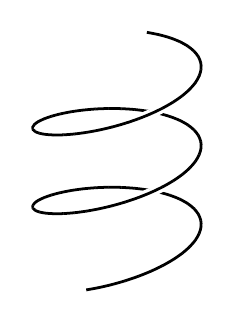
\begin{tikzpicture}[rubout/.style={/utils/exec=\tikzset{rubout/.cd,#1},
        decoration={show path construction,
        curveto code={
            \draw [white,line width=\pgfkeysvalueof{/tikz/rubout/line width}+2*\pgfkeysvalueof{/tikz/rubout/halo}]
            (\tikzinputsegmentfirst) .. controls
            (\tikzinputsegmentsupporta) and (\tikzinputsegmentsupportb)  ..(\tikzinputsegmentlast);
            \draw [line width=\pgfkeysvalueof{/tikz/rubout/line width},shorten <=-0.1pt,shorten >=-0.1pt] (\tikzinputsegmentfirst) .. controls
            (\tikzinputsegmentsupporta) and (\tikzinputsegmentsupportb) ..(\tikzinputsegmentlast);
        }}},rubout/.cd,line width/.initial=2pt,halo/.initial=0.5pt]
            \draw[rubout={line width=1pt,halo=1.2pt},decorate,
                domain=0:900,samples=101,smooth,variable=\t]
            plot({sin(\t)},\t/360,{cos(\t)});
        \end{tikzpicture}
        \caption{Intuitively, if we keep zooming in, we get a straight line on the spiral}
        \label{fig:spiral}
    \end{figure}
\end{tcolorbox}

In essence, an $n$-dimensional manifold ``looks like" $\mathbb{R}^n$ locally.

\subsection{Formal Definition of Manifolds}

The chief problem with the \hyperref[subsec:intuitive-manifolds]{intuitive introduction of manifolds} is that it depends
on having an ``ambient Euclidean space" in which our $n$-manifold lives. This introduces a great deal of extraneous
structure that is irrelevant to our purpose. Instead, we would like to view a manifold as a mathematical object in its
own right, not as a subset of some larger space. They key concept that makes this possible is that of a
\textit{topological space}.

\begin{Definition}{Continuous Mapping}{continuous-mapping}
    If $(M_1, d_1)$ and $(M_2, d_2)$ are metric spaces and $x$ is a point in $M_1$, a map $f: M_1 \rightarrow M_2$ is
    said to be \textbf{continous at $x$} if for any $\epsilon > 0$ there exists $\delta > 0$ such that
    $d_1(x, y) < \delta$ implies $d_2(f(x), f(y)) < \epsilon$ for all $y \in M_1$; and $f$ is \textbf{continuous} if it
    is continuous at every point of $M_1$\footnote{\href{https://trello.com/c/SI33o8fG}{Introduction to Topological Manifolds}, John M. Lee, 2nd, P.398}
\end{Definition}

\begin{Definition}{Image}{image}
    Let $f: X \rightarrow Y$ be a function. If $S \subset X$, the \textbf{image of $S$ under $f$}, denoted by $f(S)$, is
    the subset of $Y$ defined by\footnote{\href{https://trello.com/c/SI33o8fG}{Introduction to Topological Manifolds}, John M. Lee, 2nd, P.387}

    \begin{equation}
        f(S) = \{ y \in Y: y = f(x) \text{ for some } x \in S \}
    \end{equation}
\end{Definition}

\begin{Definition}{Preimage}{preimage}
    If $T$ is a subset of $Y$, the \textbf{preimage of $T$ under $f$} (also called the \textbf{inverse image}) is the
    subset $f^{-1}()$
\end{Definition}

    \part{Electromagnetism}

    \begin{tcolorbox}[
        parbox=false,
        enhanced,
        colback=green!5!white,
        colframe=green!75!black,
        colbacktitle=green!85!black,
        title={Why study Electromagnetism?},
        watermark graphics=砂糖-3.png,
        watermark opacity=0.3
    ]
        This question arose because I noteiced Einstein dedicated a huge portion of his famous
        \hyperlink{sr-original-paper}{Special Relativity paper} on its application in Electromagnetism.

        In fact, Einstein was trying ridiculously hard to unify his General Theory of Relativity with
        Electromagnetism\footnote{\href{https://en.wikipedia.org/wiki/Unified_field_theory}{\ldots Albert Einstein, who attempted to unify his general theory of relativity with electromagnetism \ldots}, Wikipedia}. Why?

        Relativity describes our Universe pretty good but works horribly in the microscopic world like subatomic
        particles, whereas Quantum Physics works from the opposite. Relativityis, in some sense, \textit{not complete}

        Those who are familiar with Maxwell's Equations know by heart that Electrodynamics is a beautifully
        \textit{complete} and successful theory. It has become a king of paradigm for physicists: an ideal model that
        other theories strive to emulate.

        Studying Electromagnetism is same thing as studying the standard model of Physics which shall guide my study of
        General Theory of Relativity.
    \end{tcolorbox}

    \chapter{Mathematics}
    \section{Differential Calculus}

\begin{Theorem}{
    Fundamental Lemma\footnote{\href{https://trello.com/c/byu9Pyy8}{Calculus with Analytic Geometry by George F. Simmons}, p. 680}
}{fundamental-lemma}
    Suppose that a function $z = f(x, y)$ and its partial derivatives $f_x$ and $f_y$ are defined at a point
    $(x_0, y_0)$, and also through some neighborhood of this point. Suppose further that $f_x$ and $f_y$ are continuous
    at $(x_0, y_0)$. Then the increment $\Delta z$ can be expressed in the form of

    \begin{equation}
        \Delta z = f_x(x_0, y_0)\Delta x + f_y(x_0, y_0)\Delta y + \epsilon_1\Delta x + \epsilon_2\Delta y
    \end{equation}

    where $\epsilon_1$ and $\epsilon_2 \rightarrow 0$ as $\Delta x$ and $\Delta y \rightarrow 0$
\end{Theorem}

To prove this
statement\footnote{\href{https://trello.com/c/byu9Pyy8}{Calculus with Analytic Geometry by George F. Simmons}, p. 841},
we analyze the change $\Delta z$ in 2 steps as shown in Fig.~\ref{fig:proof-fundamental-lemma}:

\begin{figure}[H]
    \centering
    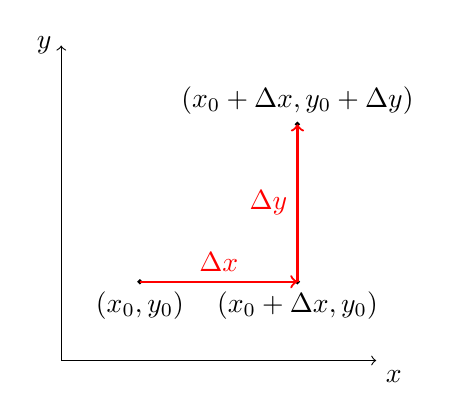
\begin{tikzpicture}
        \draw [<->] (0,4) -- (0,0) -- (4,0);
        \node [below right] at (4,0) {$x$};
        \node [left] at (0,4) {$y$};

        \draw[fill] (1,1) circle [radius=0.025];
        \draw[fill] (3,1) circle [radius=0.025];
        \draw[fill] (3,3) circle [radius=0.025];

        \node [below] at (1,1) {$(x_0, y_0)$};
        \node [below] at (3,1) {$(x_0 + \Delta x, y_0)$};
        \node [above] at (3,3) {$(x_0 + \Delta x, y_0 + \Delta y)$};

        \draw [->][thick, red] (1,1) -- node[above] {$\Delta x$} (3,1);
        \draw [->][thick, red] (3,1) -- node[left] {$\Delta y$} (3,3);
    \end{tikzpicture}
    \caption{We assume $\Delta z = f(x_0 + \Delta x, y_0 + \Delta y) - f(x_0, y_0)$ and $\Delta z = \Delta_1 z + \Delta_2 z$}
    \label{fig:proof-fundamental-lemma}
\end{figure}

\begin{enumerate}
    \item changing $x$ alone and moving from $(x_0, y_0)$ to $(x_0 + \Delta x, y_0)$, and then
    \item changing $y$ alone and moving from $(x_0 + \Delta x, y_0)$ to $(x_0 + \Delta x, y_0 + \Delta y)$
\end{enumerate}

We denote the first change in $z$ by $\Delta_1 z$, so that

\begin{equation}
    \Delta_1 z = f(x_0 + \Delta x, y_0) - f(x_0, y_0)
\end{equation}

By The Mean Value Theorem\footnote{
    \begin{Theorem}{
        The Mean Value Theorem\footnote{\href{https://trello.com/c/byu9Pyy8}{Calculus with Analytic Geometry by George F. Simmons}, p. 76}
    }{mean-value-theorem}
        Let $y = f(x)$ be a function with the following two properties:

        \begin{enumerate}
            \item $f(x)$ is continuous on the closed interval $[a, b]$; and
            \item $f(x)$ is differentiable on the open interval $(a, b)$
        \end{enumerate}

        Then there exists at least one point $c$ in the open interval $(a, b)$ such that

        \[
            f'(c) = \frac{f(b) - f(a)}{b - a}
        \]

        or equivalently,

        \[
            f(b) - f(a) = f'(c)(b - a)
        \]
    \end{Theorem}
}, we can write this as

\begin{equation}\label{eq:first-change-z-mean-val-theo}
\Delta_1 z = \Delta x f_x(x_1, y_0)
\end{equation}

where $x_1$ is between $x_0$ and $x_0 + \Delta x$. Smilary, if we denote the second part of the change in $z$ by
$\Delta_1 z$, so that

\begin{equation}
    \Delta_2 z = f(x_0 + \Delta x, y_0 + \Delta y) - f(x_0 + \Delta x, y_0)
\end{equation}

then

\begin{equation}\label{eq:second-change-z-mean-val-theo}
\Delta_2 z = \Delta y f_y(x_0 + \Delta x, y_1)
\end{equation}

where $y_1$ is between $y_0$ and $y_0 + \Delta y$.

Now as $\Delta x$ and $\Delta y \rightarrow 0$, $x_1 \rightarrow x_0$ and $y_1 \rightarrow y_0$. By the assumed
continuity of $f_x$ and $f_y$ at $(x_0, y_0)$, we can write

\begin{align}
    f_x(x_1, y_0) = f_x(x_0, y_0) + \epsilon_1 \label{eq:first-change-z-epsilon} \\
    f_y(x_0 + \Delta x, y_1) = f_y(x_0, y_0) + \epsilon_2 \label{eq:second-change-z-epsilon}
\end{align}

where $\epsilon_1$ and $\epsilon_2 \rightarrow 0$ as $\Delta x$ and $\Delta y \rightarrow 0$. Plugging
Eq.\ref{eq:first-change-z-epsilon} into Eq.\ref{eq:first-change-z-mean-val-theo} gives us

\begin{equation}
    \Delta_1 z = \Delta x\left[ f_x(x_0, y_0) + \epsilon_1 \right] = \Delta x f_x(x_0, y_0) + \Delta x\epsilon_1
\end{equation}

and similarly Eq.\ref{eq:second-change-z-epsilon} into Eq.\ref{eq:second-change-z-mean-val-theo}

\begin{equation}
    \Delta_2 z = \Delta y\left[ f_y(x_0, y_0) + \epsilon_2 \right] = \Delta y f_y(x_0, y_0) + \Delta y\epsilon_2
\end{equation}

Since we have assumed $\Delta z = \Delta_1 z + \Delta_2 z$

\begin{equation}
    \Delta z = \Delta x f_x(x_0, y_0) + \Delta x\epsilon_1 + \Delta y f_y(x_0, y_0) + \Delta y\epsilon_2 = f_x(x_0, y_0)\Delta x + f_y(x_0, y_0)\Delta y + \epsilon_1\Delta x + \epsilon_2\Delta y
\end{equation}

\qed

Now Let f(x, y, z) be a function (of three variables ! ) defined throughout some region
of three-dimensional space, and let P be a point in this region. At what rate does
f change as we move away from P in a specified direction? In the directions of
the positive x-, y-, and z-axes, we know that the rates of change off are given by
the partial derivatives CJf/CJx, CJf/CJy, and CJf/CJz. But how do we calculate the rate
of change off if we move away from P in a direction that is not a coordinate di­
rection? In analyzing this problem, we will encounter the very important concept



					of the gradient of a function.











\subsection{Gradient}



\begin{equation}
    dT = \left( \frac{\partial T}{\partial x} \right) dx + \left( \frac{\partial T}{\partial y} \right) dy + \left( \frac{\partial T}{\partial z} \right) dz
\end{equation}
\end{document}
